\documentclass[10pt,a4paper]{article}
\usepackage[margin=10mm]{geometry}
\usepackage{tikz}
%\usepackage{flowchart}
\usetikzlibrary{positioning}
\usetikzlibrary{shapes.misc}
\usetikzlibrary{shapes.geometric}
\usetikzlibrary{shapes.symbols}
\usetikzlibrary{arrows}
\usetikzlibrary{fit}
\usetikzlibrary{backgrounds}

\begin{document}
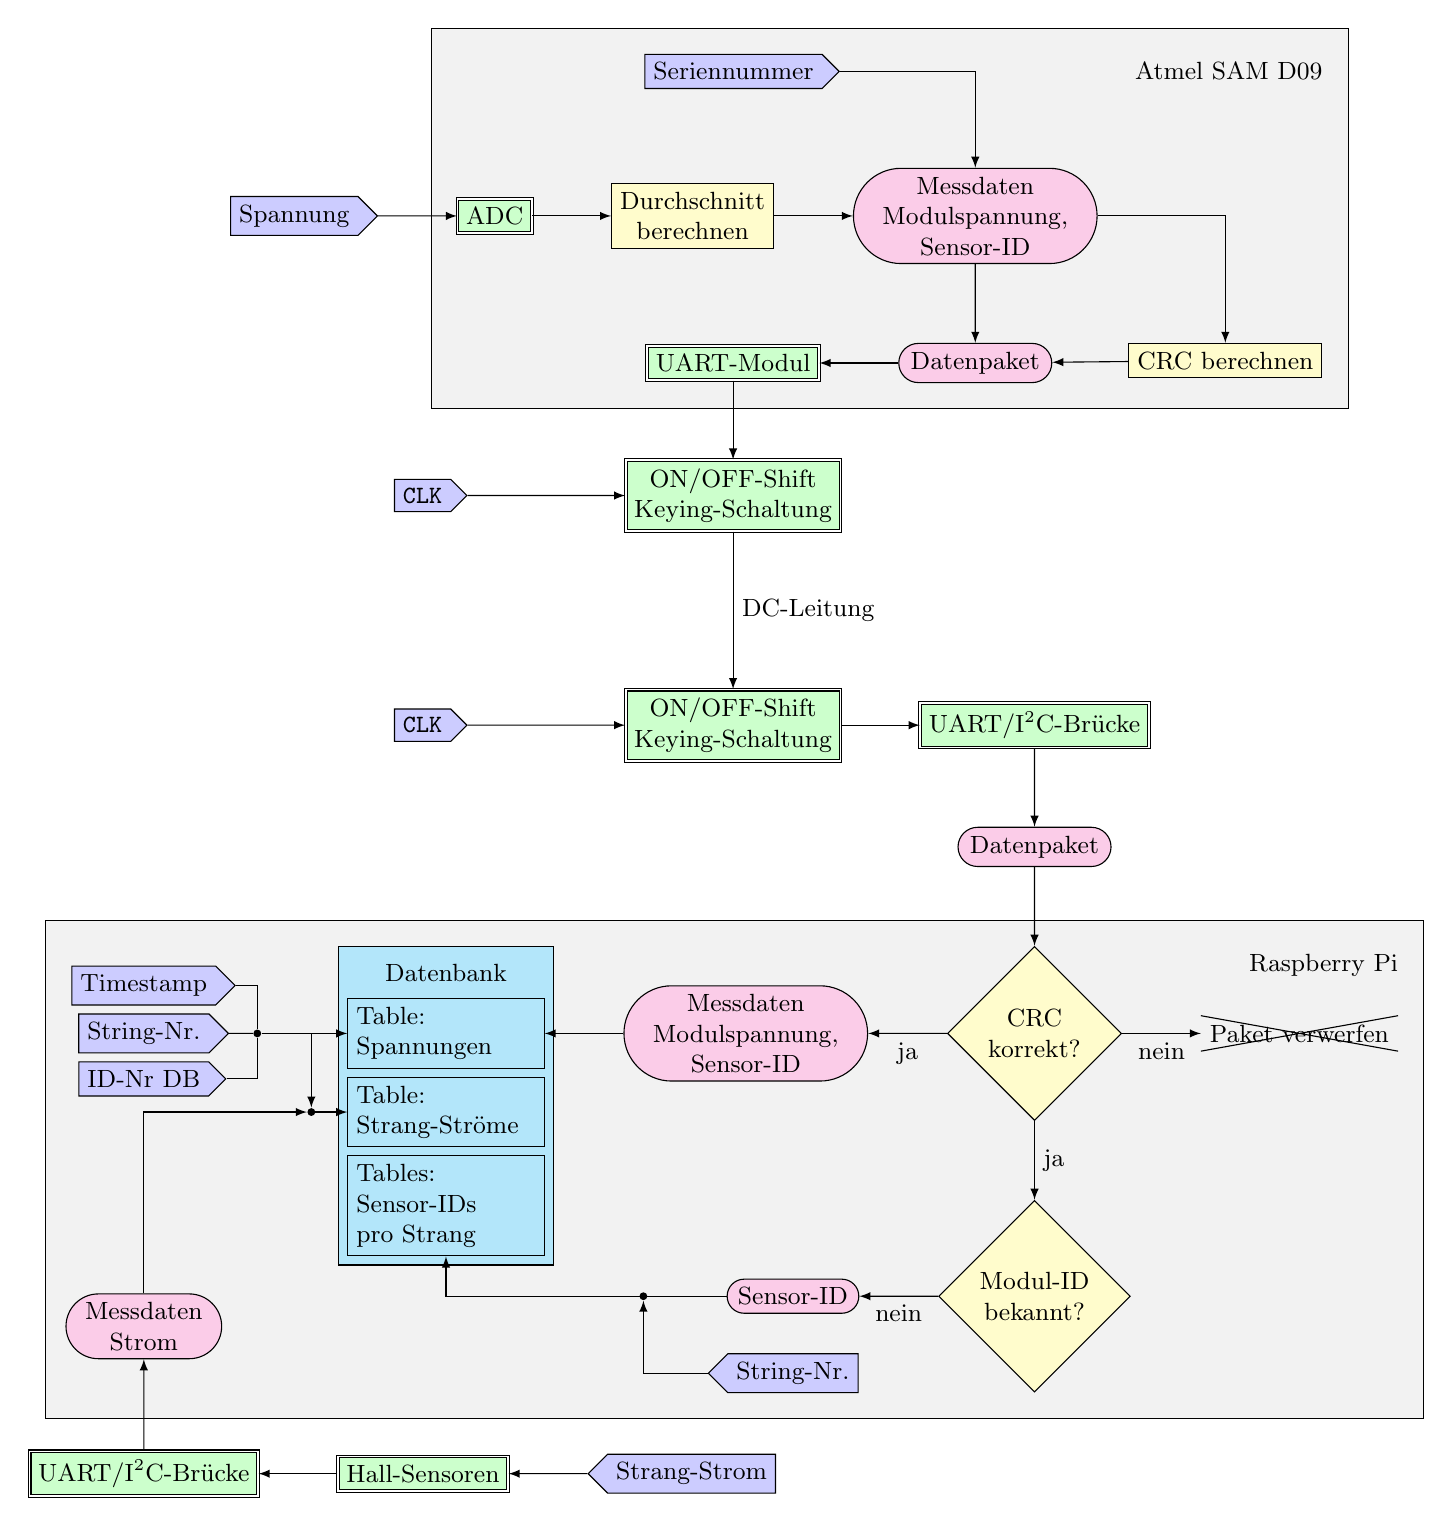
\begin{tikzpicture}[%
        %rounded corners,
        align=center,
        %node distance = 5mm,
    ]
    \small
    %\begin{scope}[x={(0mm,0.95\textwidth)},y={(0mm,50mm)}]

    %\draw [help lines] (0,0) grid (10,-15);

    %\node at (1,1) [above=2pt+3pt,draw] {above};

    \begin{scope}[
        every node/.style = draw,
        terminal/.append style={rounded rectangle,fill=magenta!20},
        sign/.style={fill=blue!20},         % custom signal style
        circ/.style={double,fill=green!20}, % circuitry
        proc/.style={fill=yellow!20},       % process/activity
        stor/.style={fill=cyan!30},         % storage
    ]
        \node (voltage)   [sign,signal,signal to=east] at (0,0)     {Spannung};

        % uC on Sensor
        \node (ADCVolt)   [circ,right=of voltage]                        {ADC};
        \node (avg)       [proc,right=of ADCVolt,align=center]           {Durchschnitt\\berechnen};
        \node (data)      [terminal,right=of avg,align=center]                   {Messdaten\\Modulspannung,\\Sensor-ID};
        \node (id)        [sign,signal,signal to=east,above left=of data] {Seriennummer};
        \node (crc)       [proc,below right=of data]                     {CRC berechnen};
        \node (package)   [terminal,below=of data]                  {Datenpaket};
        \node (uart)      [circ,left=of package]                         {UART-Modul};

        \node (oosk1)     [circ,below=of uart,align=center]                   {ON/OFF-Shift \\Keying-Schaltung};
        \node (clk1)      [sign,signal,signal to=east,left=2cm of oosk1]      {\texttt{CLK}};
        \node (oosk2)     [circ,below=20mm of oosk1,align=center]             {ON/OFF-Shift \\Keying-Schaltung};
        \node (clk2)      [sign,signal,signal to=east,left=2cm of oosk2]      {\texttt{CLK}};
        \node (bridge)    [circ,right=of oosk2]                                    {UART/I\textsuperscript{2}C-Br\"ucke};
        \node (package2)  [terminal,below=of bridge] {Datenpaket};

        % Raspi
        \node (crc2)      [proc,align=center,diamond,below=of package2]                          {CRC\\korrekt?};
        \node (discard)   [cross out,right=of crc2]                                            {Paket verwerfen};
        \node (data2)     [terminal,left=of crc2,align=center]                                 {Messdaten\\Modulspannung,\\Sensor-ID};
        \node (dbVolts)   [left=of data2,text width=7em,align=left,minimum width=7.5em]     {Table:\\ Spannungen\\};
        \node (dbCurr)    [below=1mm of dbVolts,text width=7em,align=left,minimum width=7.5em] {Table:\\ Strang-Str\"ome\\};
        \node (dbIDs)     [below=1mm of dbCurr,text width=7em,align=left,minimum width=7.5em]  {Tables:\\ Sensor-IDs \\ pro Strang};

        \node (newID)     [proc,align=center,diamond,below=of crc2]                          {Modul-ID\\bekannt?};
        \node (sensorID)  [terminal,left=of newID] {Sensor-ID};
        \node (stringNr2) [sign,signal,signal to=west,below=5mm of sensorID] {String-Nr.};

        \node (stringNr)  [sign,signal,signal to=east,left=15mm of dbVolts]       {String-Nr.};
        \node (timestamp) [sign,signal,signal to=east,above=1mm of stringNr] {Timestamp};
        \node (dbID)      [sign,signal,signal to=east,below=1mm of stringNr] {ID-Nr DB};

        \node (dataCurr) [terminal,below=25mm of dbID,align=center] {Messdaten\\Strom};

        \node (bridge2) [circ,below=45mm of dbID] {UART/I\textsuperscript{2}C-Br\"ucke};
        \node (hall)    [circ,right=of bridge2] {Hall-Sensoren};
        \node (current) [sign,signal,signal to=west,right=of hall]         {Strang-Strom};
    \end{scope}

    \begin{scope}
        % Need to have this inside  a separate scope so that
        % its border does not get drawn.
        \node (db)        [above=1mm of dbVolts,align=left] {Datenbank};
        \node (dbSignals) [circle,inner sep=1pt,fill=black,right=3mm of stringNr] { };
        \node (dbSignals2)[circle,inner sep=1pt,fill=black,left=4mm of dbCurr] { };
        \node (dbSignals3)[circle,inner sep=1pt,fill=black,left=of sensorID] { };
    \end{scope}

    \begin{scope}[on background layer]
        \node (uCSensor) [%
            draw,
            fill=gray!10,
            inner sep=1em,
            fit=(ADCVolt) (avg) (data) (id) (crc) (package) (uart),
            align=right,
            text height=1em,
        ] {Atmel SAM D09};
        \node (rasPi) [%
            draw,
            fill=gray!10,
            inner sep=1em,
            fit=(stringNr) (timestamp) (dbID) (crc2) (newID) (discard) (stringNr2),
            align=right,
            text height=1em,
        ] {Raspberry Pi};
        \node (database) [%
            draw,
            fill=cyan!30,
            fit=(dbVolts) (dbCurr) (dbIDs) (db),
        ] { };
    \end{scope}


    \begin{scope}[
        %every node/.style={ },
    ]
        \draw[-latex] (voltage) -- (ADCVolt);
        \draw[-latex] (ADCVolt) -- (avg);
        \draw[-latex] (id) -| (data);
        \draw[-latex] (avg) -- (data);
        \draw[-latex] (data) -| (crc);
        \draw[-latex] (crc) -- (package);
        \draw[-latex] (data) -- (package);
        \draw[-latex] (package) -- (uart);
        \draw[-latex] (uart) -- (oosk1);
        \draw[-latex] (clk1) -- (oosk1);
        \draw[-latex] (clk2) -- (oosk2);
        \draw[-latex] (oosk1) --  node[midway, anchor = west] {DC-Leitung} (oosk2);
        \draw[-latex] (oosk2) -- (bridge);
        \draw[-latex] (bridge) -- (package2);
        \draw[-latex] (package2) -- (crc2);
        \draw[-latex] (crc2) -- node[anchor=north] {nein} (discard);
        \draw[-latex] (crc2) -- node[anchor=north] {ja} (data2);
        \draw[-latex] (data2) -- (dbVolts);
        \draw[-] (stringNr) -- (dbSignals);
        \draw[-] (timestamp) -| (dbSignals);
        \draw[-] (dbID) -| (dbSignals);
        \draw[-latex] (dbSignals) -- (dbVolts);
        \draw[-latex] (dbSignals) -| (dbSignals2);
        \draw[-latex] (dbSignals2) |- (dbCurr);
        \draw[-latex] (crc2) -- node[anchor=west,align=right] {ja} (newID);
        \draw[-latex] (newID) -- node[anchor=north] {nein} (sensorID);
        \draw[-latex] (sensorID) -| (dbIDs);
        \draw[-latex] (stringNr2) -| (dbSignals3);
        \draw[-latex] (current) -- (hall);
        \draw[-latex] (hall) -- (bridge2);
        \draw[-latex] (bridge2) -- (dataCurr);
        \draw[-latex] (dataCurr) |- (dbSignals2);
        %\draw[-latex] (current) -| (dbSignals2);
        %\draw[-latex] (dbSignals3) |- (dbCurr);
    \end{scope}

\end{tikzpicture}

\end{document}
